\documentclass{beamer}
\usepackage[utf8]{inputenc}

\usetheme{Madrid}
\usecolortheme{default}
\usepackage{amsmath,amssymb,amsfonts,amsthm}
\usepackage{mathtools}
\usepackage{txfonts}
\usepackage{tkz-euclide}
\usepackage{listings}
\usepackage{adjustbox}
\usepackage{array}
\usepackage{gensymb}
\usepackage{tabularx}
\usepackage{gvv}
\usepackage{lmodern}
\usepackage{circuitikz}
\usepackage{tikz}
\usepackage{graphicx}

\setbeamertemplate{page number in head/foot}[totalframenumber]

\usepackage{tcolorbox}
\tcbuselibrary{minted,breakable,xparse,skins}



\definecolor{bg}{gray}{0.95}
\DeclareTCBListing{mintedbox}{O{}m!O{}}{%
  breakable=true,
  listing engine=minted,
  listing only,
  minted language=#2,
  minted style=default,
  minted options={%
    linenos,
    gobble=0,
    breaklines=true,
    breakafter=,,
    fontsize=\small,
    numbersep=8pt,
    #1},
  boxsep=0pt,
  left skip=0pt,
  right skip=0pt,
  left=25pt,
  right=0pt,
  top=3pt,
  bottom=3pt,
  arc=5pt,
  leftrule=0pt,
  rightrule=0pt,
  bottomrule=2pt,
  toprule=2pt,
  colback=bg,
  colframe=orange!70,
  enhanced,
  overlay={%
    \begin{tcbclipinterior}
    \fill[orange!20!white] (frame.south west) rectangle ([xshift=20pt]frame.north west);
    \end{tcbclipinterior}},
  #3,
}
\lstset{
    language=C,
    basicstyle=\ttfamily\small,
    keywordstyle=\color{blue},
    stringstyle=\color{orange},
    commentstyle=\color{green!60!black},
    numbers=left,
    numberstyle=\tiny\color{gray},
    breaklines=true,
    showstringspaces=false,
}
%------------------------------------------------------------
%This block of code defines the information to appear in the
%Title page
\title %optional
{1.4.21}
\date{september 11,2025}
%\subtitle{A short story}

\author % (optional)
{EE25BTECH11006 - ADUDOTLA SRIVIDYA}

\begin{document}

\frame{\titlepage}

\begin{frame}{Question}
Find the coordinates of the point which divides the line segment joining
$
(1,-2,3), \quad (3,4,-5)
$
in the ratio
\begin{enumerate}[label=(\alph*)]
    \item \(2 : 3\) internally
    \item \(2 : 3\) externally
\end{enumerate}
\end{frame}

\begin{frame}{Given Information}
Given vector \vec{A}:
\begin{align}
\myvec{ 1 \\ -2 \\ 3 }
\end{align}
Given vector \vec{B}:
\begin{align}
\myvec{ 3 \\ 4 \\ -5 }
\end{align}
\end{frame}

\begin{frame}{Required Formulae}
Internal division:
\begin{align}
\vec{P} = \frac{kB+A}{k+1}
\end{align}

External division:
\begin{align}
\vec{Q} = \frac{kB-A}{k-1}
\end{align}
\end{frame}

\begin{frame}{Solution - Internal}
\begin{align}
\vec{P} = \frac{\dfrac{2}{3}\myvec{3 \\ 4 \\ -5} + \myvec{1 \\ -2 \\ 3}}{\dfrac{5}{3}} 
\end{align}
\begin{align}
    \vec{P} = \frac{\myvec{2 \\ \dfrac{8}{3} \\ \dfrac{-10}{3}} + \myvec{1 \\ -2 \\ 3}}{\dfrac{5}{3}}
= \frac{\myvec{3 \\ \dfrac{2}{3} \\ \dfrac{-1}{3}}}{\dfrac{5}{3}}
= \myvec{\tfrac{9}{5} \\ \tfrac{2}{5} \\ \tfrac{-1}{5}}
\end{align}
\end{frame}

\begin{frame}{Solution - External}
\begin{align}
\vec{Q} = \frac{\dfrac{2}{3}\myvec{3 \\ 4 \\ -5} - \myvec{1 \\ -2 \\ 3}}{\dfrac{5}{3}}
\end{align}
\begin{align}
\vec{Q} = \frac{\myvec{2 \\ \dfrac{8}{3} \\ \dfrac{-10}{3}} - \myvec{1 \\ -2 \\ 3}}{\dfrac{-1}{3}}
= \frac{\myvec{1 \\ \dfrac{14}{3} \\ \dfrac{-19}{3}}}{\dfrac{-1}{3}}
= \myvec{-3 \\ -14 \\ 19}
\end{align}

\end{frame}

\begin{frame}[fragile]{Python Code-Plot}
\begin{lstlisting}
import matplotlib.pyplot as plt
from mpl_toolkits.mplot3d import Axes3D
A = (1, -2, 3)
B = (3, 4, -5)
P = (
    (2*B[0] + 3*A[0]) / 5,
    (2*B[1] + 3*A[1]) / 5,
    (2*B[2] + 3*A[2]) / 5
)
Q = (
    (2*B[0] - 3*A[0]) / (2-3),
    (2*B[1] - 3*A[1]) / (2-3),
    (2*B[2] - 3*A[2]) / (2-3)
)
print("Internal Division Point:", P)
print("External Division Point:", Q)
\end{lstlisting}
\end{frame}

\begin{frame}[fragile]{Python Code-Plot}
\begin{lstlisting}
fig = plt.figure(figsize=(8,8))
ax = fig.add_subplot(111, projection='3d')
ax.plot([A[0], B[0]], [A[1], B[1]], [A[2], B[2]], color='blue')
def plot_point(pt, label, color):
    ax.scatter(*pt, color=color, s=60)
    ax.text(pt[0], pt[1], pt[2], f"{label}{pt}", fontsize=10)
plot_point(A, "A", "red")
plot_point(B, "B", "red")
plot_point(P, "P", "green")
plot_point(Q, "Q", "purple")
ax.set_xlabel('X-axis')
ax.set_ylabel('Y-axis')
ax.set_zlabel('Z-axis')
ax.set_title('3D Division of Line Segment')


\end{lstlisting}
\end{frame}

\begin{frame}[fragile]{Python Code-Plot}
\begin{lstlisting}
ax.set_xlim(-4, 4)
ax.set_ylim(-15, 5)
ax.set_zlim(-5, 19)

plt.savefig("Figs/graph.png")
plt.show()
\end{lstlisting}
\end{frame}


\begin{frame}[fragile]{Python ctypes Call}
\begin{lstlisting}
import ctypes

lib = ctypes.CDLL('./mat1.so')

lib.sectionFormula.argtypes = [
    ctypes.POINTER(ctypes.c_float),
    ctypes.POINTER(ctypes.c_float),
    ctypes.c_float,
    ctypes.c_float,
    ctypes.POINTER(ctypes.c_float)
]
\end{lstlisting}
\end{frame}

\begin{frame}[fragile]{Python ctypes Call}
\begin{lstlisting}
lib.sectionFormula.restype = None
lib.sectionFormulaExternal.argtypes = [
    ctypes.POINTER(ctypes.c_float),
    ctypes.POINTER(ctypes.c_float),
    ctypes.c_float,
    ctypes.c_float,
    ctypes.POINTER(ctypes.c_float)
]
lib.sectionFormulaExternal.restype = None
p1 = (ctypes.c_float * 3)(1.0, -2.0, 3.0)
p2 = (ctypes.c_float * 3)(3.0, 4.0, -5.0)
res_internal = (ctypes.c_float * 3)()
res_external = (ctypes.c_float * 3)()
m = 2.0
n = 3.0
\end{lstlisting}
\end{frame}

\begin{frame}[fragile]{Python ctypes Call}
\begin{lstlisting}
lib.sectionFormula(p1, p2, m, n, res_internal)
lib.sectionFormulaExternal(p1, p2, m, n, res_external)

print("Internal division (2:3): [{:.2f}, {:.2f}, {:.2f}]".format(
    res_internal[0], res_internal[1], res_internal[2]
))

print("External division (2:3): [{:.2f}, {:.2f}, {:.2f}]".format(
    res_external[0], res_external[1], res_external[2]
))
\end{lstlisting}
\end{frame}
\begin{frame}[fragile]{C Code}
\begin{lstlisting}
void sectionFormula(float p1[3], float p2[3], float m, float n,
float res[3]) {
    res[0] = (m * p2[0] + n * p1[0]) / (m + n);
    res[1] = (m * p2[1] + n * p1[1]) / (m + n);
    res[2] = (m * p2[2] + n * p1[2]) / (m + n);
}

void sectionFormulaExternal(float p1[3], float p2[3], float m, 
float n, float res[3]) {
    res[0] = (m * p2[0] - n * p1[0]) / (m - n);
    res[1] = (m * p2[1] - n * p1[1]) / (m - n);
    res[2] = (m * p2[2] - n * p1[2]) / (m - n);
}
\end{lstlisting}
\end{frame}

\begin{frame}{Plot}
\begin{figure}
\centering
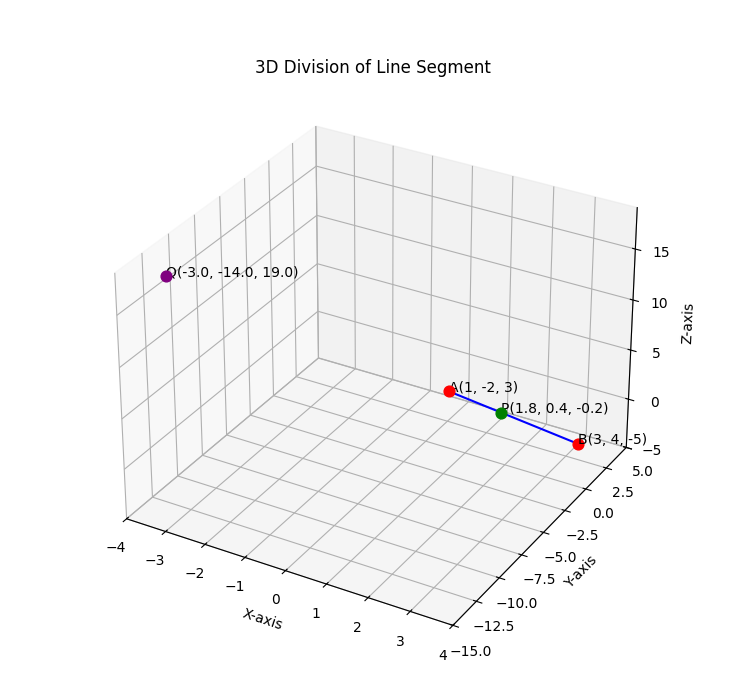
\includegraphics[width=0.6\linewidth]{figs/fig1.png}
\caption{3D Plot of points \(A, B, P, Q\)}
\label{fig:graph}
\end{figure}
\end{frame}
\end{document}